\chapter{零和博弈}
零和博弈(zero-sum game)刻画的是两名玩家利益完全相反的情形：一方的损失正是另一方的收益。许多双人竞技项目和室内游戏都可以这样理解。第1章讨论的组合博弈，也属于零和博弈。

在零和博弈中，不论出现哪一个结果，所有玩家的收益之和都为零。若 \(B=-A\) ，则 \(m \times  n\) 双矩阵博弈(bimatrix game)$ (A, B) $就是零和博弈。此时整个博弈已经由行玩家的收益矩阵 \(A\) 完全决定，因此通常称为矩阵博弈(matrix game)。矩阵博弈当然仍可作为双矩阵博弈来分析，但零和结构带来了一些一般双矩阵博弈没有的强性质。本章主要讨论这些性质：

\begin{itemize}
\item 在零和博弈中，均衡策略就是极大极小策略(max-min strategy)；它使玩家在最坏情况下的期望效用(expected payoff)尽可能高，因此不依赖于对手实际采用的行动。

\item 所有均衡给玩家带来的收益都相同，而且这个收益唯一确定，称为博弈的值。

\item 如果玩家有多个均衡策略，这些策略可以相互替换，并能与对方任意均衡策略配对形成均衡。此外，每个玩家的均衡策略集都是凸集(convex set)。
\end{itemize}

除了这些特殊性质，本书还单独安排一章讨论零和博弈，原因有三点：

\begin{itemize}
\item 从历史上看，冯·诺伊曼(1928 年)关于零和博弈的主要结果，早于纳什(1951 年)针对一般收益博弈提出的均衡概念。

\item “没有偏离动机”这一均衡思想，在零和博弈中有更强的形式：玩家甚至可以公开自己的策略，而不会因此处于劣势。硬币匹配博弈和石头剪刀布博弈已经说明，这需要混合策略(mixed strategy)的概念(见图~\ref{fig:3.12})。当然，零和博弈并不总是需要混合策略；例如第 1 章和第 4 章中的完美信息博弈就不需要。如果某个玩家只有两种策略，该博弈还是占优可解的，见练习~\ref{exer:8.2}。

\item 本章在数学上相对自洽，并用很短的篇幅独立证明冯·诺伊曼的极小极大定理(minimax theorem)。根据命题~\ref{prop:8.3}，该定理等价于零和博弈中均衡的存在性。极小极大定理没有布劳威尔不动点定理那么强，也略弱于线性规划对偶定理(linear programming duality)，但它在第 12 章证明相关均衡存在性时会再次派上用场。
\end{itemize}

第~\ref{sec:8.2} 节以足球点球为例介绍零和博弈，并说明怎样用图形方法找出极大极小策略(图~\ref{fig:8.2} 和图~\ref{fig:8.3})。

第~\ref{sec:8.3} 节讨论零和博弈的主要性质。核心概念是极大极小策略：玩家选择一种通常为混合的策略，使自己在对手所有可能反应下的最低期望效用尽可能高。这种思路看起来有些保守，原则上可用于任何博弈；但在零和博弈中，对手确实会把你的收益压到最低，因此这种推理正是合理的。

在矩阵博弈中，行玩家希望最大化自己的收益；同一个数对列玩家来说则是要尽量压低的成本(cost)。换句话说，列玩家希望最小化行玩家的收益。用成本来表述时，行玩家的极大极小策略，在列玩家一侧就对应极小极大策略(min-max strategy)：列玩家选择一种策略，使得无论行玩家如何反应，自己可能承担的最大成本都尽可能小。如果行玩家的极大极小收益等于列玩家的极小极大成本，那么这两种策略共同构成一个均衡；反过来，零和博弈的均衡也正是这样的一对策略(命题~\ref{prop:8.3})。由于有限博弈一定存在均衡，上述“极大极小 = 极小极大”的等式必然成立，这就是冯·诺伊曼(1928)的极小极大定理(定理~\ref{theo:8.4})。该定理还给出一个唯一确定的均衡结果：行玩家在均衡中的收益，也就是列玩家的成本，是一个唯一的数，称为博弈的值。

第~\ref{sec:8.4} 节给出极小极大定理的一个简短证明，不依赖均衡存在性定理。证明把两个相关的优化问题联系起来；这两个问题是一对对偶线性规划(linear programming duality)的特殊情形。我们只处理这个特殊情形，并用归纳法直接证明二者有相同的最优值。

在零和博弈中，均衡策略与按自身收益定义的极大极小策略一致，也称为最优策略(optimal strategy)。它不依赖对手实际如何行动，这是一个很强的性质。第~\ref{sec:8.5} 节将继续讨论最优策略的其他性质。

\section{ 预备知识和学习目标}\label{sec:8.1}

本章需要用到第6章中双矩阵博弈和混合策略的定义，以及基本的矩阵运算(matrix multiplication)和向量线性不等式。第~\ref{sec:8.4} 节证明极小极大定理时，还会用到连续函数在紧集(compact set)上能取到最小值和最大值这一事实。

学习本章后，你应该能够:

\begin{itemize}
\item 解释极大极小策略的概念及其对零和博弈的重要性，并将其应用于给定的博弈中。
\item 像练习~\ref{exer:8.1}那样，在小型矩阵博弈中找出极大极小策略和极小极大策略，并利用“极大极小值 = 极小极大值”定理，通过期望效用的下包络或上包络找到更容易计算的一方策略。
\item 陈述并证明零和博弈中均衡的存在性与极小极大定理的等价性(命题~\ref{prop:8.3})。
\item 陈述零和博弈的主要性质：最优策略与对手行动无关，并说明由此带来的结论，包括唯一的博弈值、策略可交换性和均衡策略集的凸性。
\item 解释第~\ref{sec:8.3} 节中极小极大定理归纳证明背后的主要思想。
\end{itemize}

\section{示例:点球大战}\label{sec:8.2}

零和博弈是满足 \(B = -A\) 的双矩阵博弈 \((A,B)\)。由于它完全由行玩家 \(\mathrm{I}\) 的收益矩阵 \(A\) 决定，也称为收益矩阵为 \(A\) 的矩阵博弈。当两名玩家分别选择行 \(i\) 和列 \(j\) 时，矩阵元素 \({a}_{ij}\) 可理解为玩家II支付给玩家I的数额；因此它是玩家II希望最小化的成本，面对混合策略时也按期望成本来理解。玩家I称为最大化者(maximizer)，玩家II称为最小化者(minimizer)。

图~\ref{fig:8.1}把足球点球写成前锋和守门员之间的零和博弈。为简单起见，设前锋只有两种策略 \(L\) 和 \(R\) ，即射向左下角或右下角；守门员有三种策略 \(l,w,r\) ，其中 \(l\) 和 \(r\) 表示立即扑向左侧或右侧， \(w\) 表示先等待、观察球的方向后再扑。图~\ref{fig:8.2}给出一个例子：每个单元格中的数是前锋进球的概率。前锋(玩家I)希望这个概率尽量高，守门员(玩家II)希望它尽量低，所以只用前锋的收益就能描述整个博弈。下文把最大化者记为“Max”，最小化者记为“min”(列玩家仍按惯例用小写字母表示)。

\begin{figure}
    \centering
    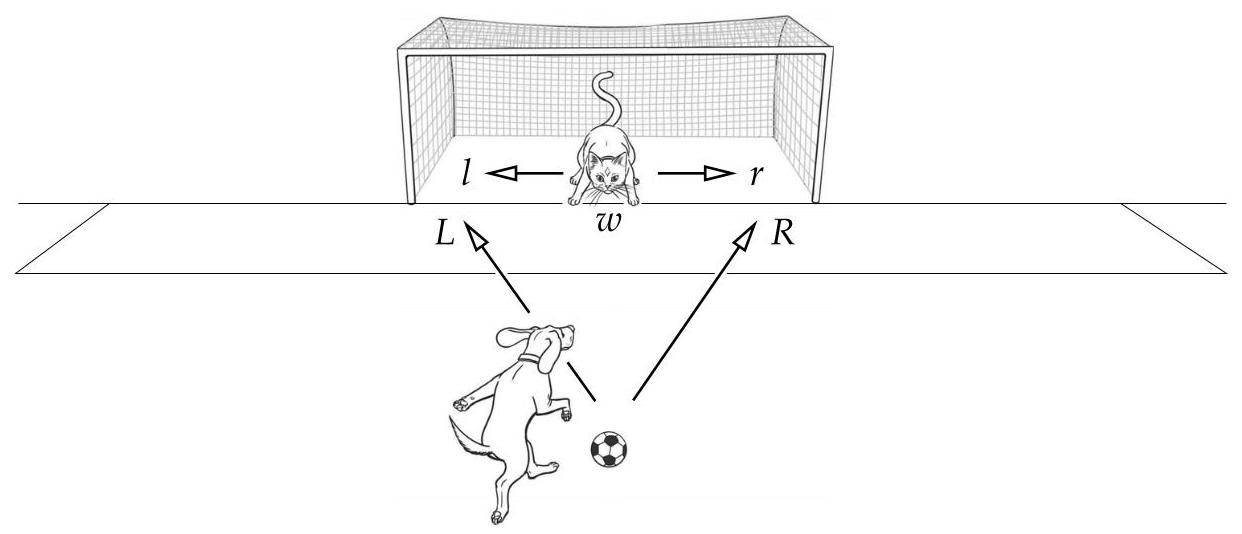
\includegraphics[width=0.8\linewidth]{images/ch08-fig01.jpg}
    \caption{足球点球大战中前锋和守门员的策略。除了向左或向右跳跃，守门员还可以等待$(w)$。练习~\ref{exer:8.1}中考虑了前锋向中间射门的额外策略。}
    \label{fig:8.1}
\end{figure}

这里的收益是进球概率，对玩家I是收益，对玩家II是成本。由于概率的期望仍是概率，它天然满足期望效用函数(expected-utility function)的要求；这也是一个把期望效用直接解释为概率的实际例子，见图~\ref{fig:5.1}。在一般零和博弈中，收益和成本未必来自概率，但仍假定它们能代表两名玩家对随机结果的期望偏好。这个假定比非零和博弈更强，因为在非零和博弈中，两名玩家的收益可以分别调整，以反映不同的风险态度。

图~\ref{fig:8.2}左上方把该博弈写成双矩阵博弈，每个单元格列出两个收益，并像前面一样用方框标出纯策略最优反应。右上方则给出更简洁的矩阵博弈形式，每个单元格只保留一个数字。方框表示最大化者的最优反应收益，圆圈表示最小化者的最优反应成本。两种写法表达的信息相同，但矩阵博弈的写法更省。

最优反应显示，这个博弈没有纯策略均衡。从点球场景本身也很容易看出：守门员最好扑向球要去的角落，而前锋则更愿意把球踢向守门员扑反的方向。因此我们必须寻找混合均衡；主动随机化对双方都有价值。

我们先像求解普通双矩阵博弈那样求这个博弈的均衡，只是现在只需关注玩家I的效用。用“门柱图”(goalpost method)来分析点球博弈正好贴切。图~\ref{fig:8.2}下方画出玩家I的期望效用：横轴是玩家I选择 \(R\) 的概率 \(p\)，三条直线分别对应玩家II的纯策略 \(l,w,r\)。这些效用对玩家II来说就是成本，所以玩家II的最优反应成本由三条直线的最小值给出，也就是粗线标出的下包络(lower envelope)。下包络上有两个交点： \(p = \frac{1}{3}\) 时， \(l\) 与 \(w\) 的直线相交； \(p = \frac{3}{5}\) 时， \(w\) 与 \(r\) 的直线相交。用差分技巧(difference trick)可以很快算出这些点。在这里看成本或看效用都一样，因为差值的绝对值相同。比如， \(l\) 和 \(w\) 在 \(L\) 行的差为0.2，在 \(R\) 行的差为0.4，所以 \(L\) 与 \(R\) 应按 \({0.4} : {0.2}\) 的比例混合，即 \(p = \frac{1}{3}\)，此时玩家I在面对 \(l\) 和 \(w\) 时无差异(indifference)。同理可得到 \(p = \frac{3}{5}\) 时， \(w\) 和 \(r\) 之间的无差异条件。


\begin{figure}
    \centering
    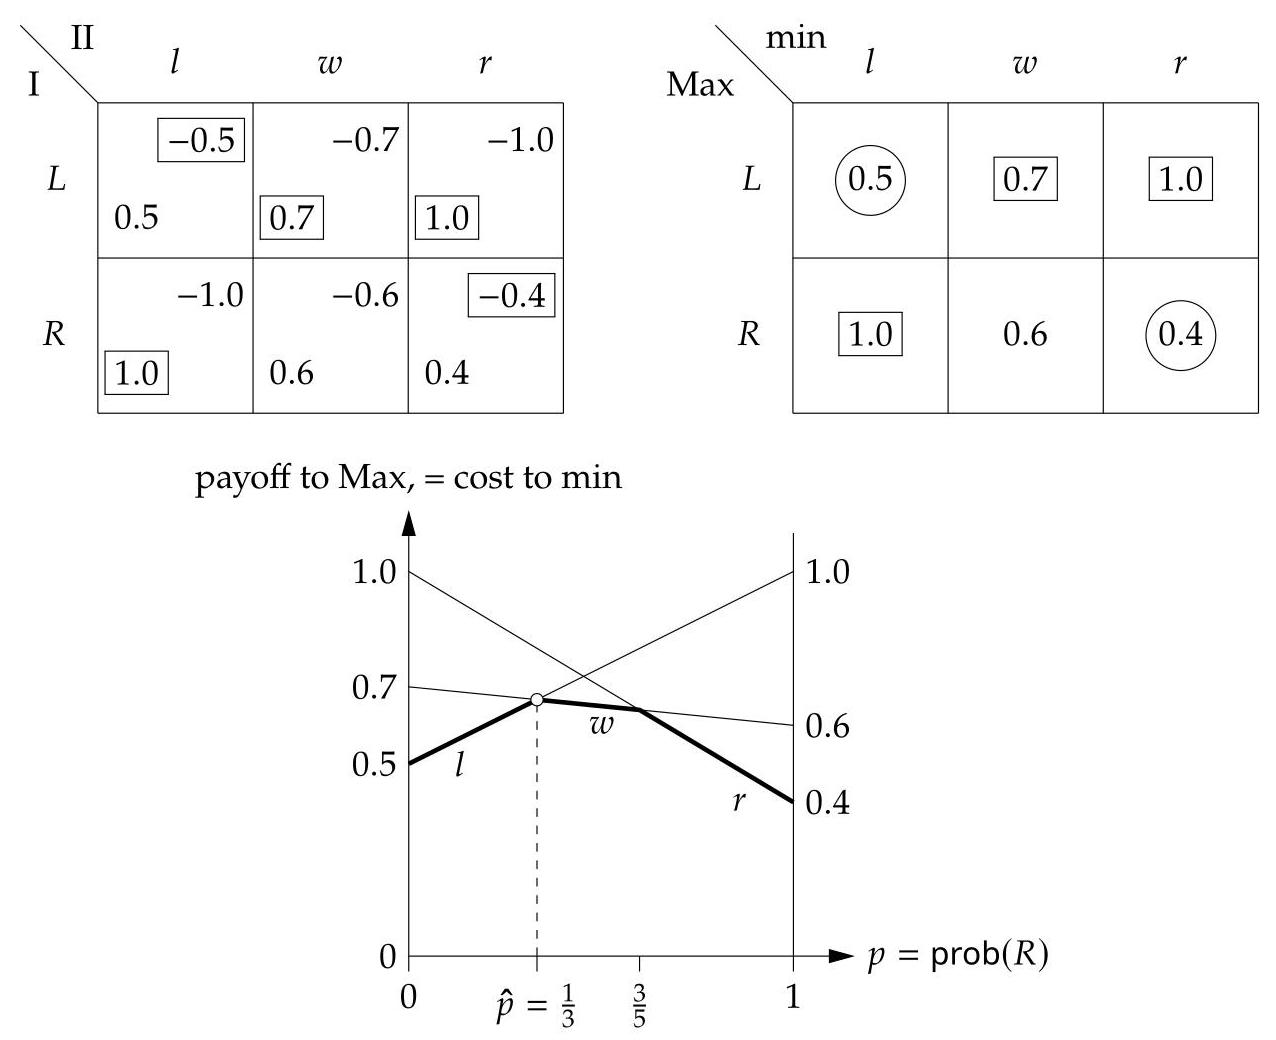
\includegraphics[width=0.8\linewidth]{images/ch08-fig02.jpg}
    \caption{左上方:点球博弈作为一个零和双矩阵博弈，得分概率作为前锋(玩家I)的效用，而这是守门员(玩家II)效用的负值。右上方:同样的博弈表示为矩阵博弈，只显示了最大值点的效用，而这是最小值点的成本。方框表示最大值点的最优反应效用，圆圈表示最小值点的最优反应(最小)成本。下方:作为最大值点混合策略$(1-p, p)$的函数，最优反应成本的下包络。对于 \(p = \widehat{p} = \frac{1}{3}\) ，这是他的极大极小策略。}
    \label{fig:8.2}
\end{figure}




因此，玩家II面对混合策略$(1-p, p)$时的最优反应如下：当 \(0 \leq  p \leq  \frac{1}{3}\) 时选 \(l\)；当 \(\frac{1}{3} \leq  p \leq  \frac{3}{5}\) 时选 \(w\)；当 \(\frac{3}{5} \leq  p \leq  1\) 时选 \(r\)。只有在 \(p = \frac{1}{3}\) 和 \(p = \frac{3}{5}\) 时，玩家II才可能混合；而只有第一种情形，也就是 \(l\) 和 \(w\) 同为最优反应时，才能反过来使玩家I无差异。于是得到该博弈唯一的混合均衡 \(\left( {\left( {\frac{2}{3},\frac{1}{3}}\right) ,\left( {\frac{1}{6},\frac{5}{6},0}\right) }\right)\) 。在这个均衡下，三列 \(l,w,r\) 的期望成本分别为 \(\frac{2}{3},\frac{2}{3},\frac{4}{5}\)，所以玩家II只给成本最低的列 \(l\) 和 \(w\) 正概率。两行的期望效用均为 \(\frac{2}{3}\)。该博弈唯一的均衡效用，就是定理~\ref{theo:8.4}中所说的博弈值。

到这里为止，分析方法和双矩阵博弈并没有本质区别。现在换成玩家I自己的视角：把玩家I的期望效用看作其混合策略 \(x = \left( {1 - p,p}\right)\) 的函数，并关注它的下包络。这个下包络表示，在玩家II各种可能反应下，玩家I能保证得到的最差期望效用。事实上，只需考虑玩家II的纯策略反应即可(也见命题~\ref{prop:8.2})。也就是说，给定混合策略 \(x\) 后，最小值会在最小化者的某个纯策略反应中达到；在这里就是列 \(l,w,r\) 中的一列。

如果玩家I想保证自己的最差收益尽可能高，就应选择合适的 \(p\) 来最大化下包络。图~\ref{fig:8.2}中的虚线显示，这个最大值在 \(\widehat{p} = \frac{1}{3}\) 处取得。策略 \(\widehat{x} = \left( {1 - \widehat{p},\widehat{p}}\right)\) 称为最大化者的极大极小策略；在图形上，它就是下包络的最高点。“帽子”符号 \(\widehat{x}\) 可以帮助记住这个峰值位置。

极大极小策略 \(\left( {1 - \widehat{p},\widehat{p}}\right)\) 对应下包络上的一个交点。另一个交点 \(p = \frac{3}{5}\) 给最大化者的收益更低，因为最优反应线 \(w\) 从 \(\frac{1}{3}\) 到 \(\frac{3}{5}\) 向下倾斜。因此， \(p = \frac{3}{5}\) 不是极大极小策略。命题~\ref{prop:8.3}将说明，在零和博弈中，均衡策略与极大极小策略相同。所以不同于一般双矩阵博弈，我们不需要再把 \(p = \frac{3}{5}\) 当作候选均衡策略去检验。

极大极小收益定义明确，并且不依赖玩家II最后采取哪一个行动，因为我们已经把玩家II所有可能反应中的最小值考虑进去了。这个最大化后的最差收益是唯一的，但实现它的极大极小策略 \(\widehat{x}\) 可能不唯一。图~\ref{fig:8.3}给出一个例子： \(L\) 和 \(R\) 在列 \(w\) 中的收益都为0.6，因此它们都是对 \(w\) 的最优反应；按定义~\ref{def:6.7}，这个博弈是退化的。此时下包络在任意 \(\widehat{p} \in  \left\lbrack  {\frac{1}{5},\frac{2}{3}}\right\rbrack\) 处都达到最大值0.6，于是这些点都给出极大极小策略 \(\widehat{x} = \left( {1 - \widehat{p},\widehat{p}}\right)\)。区间两个端点仍可分别通过 \(l\) 与 \(w\)、 \(w\) 与 \(r\) 的无差异条件，用差分技巧算出。另一方面，例如当 \(\widehat{p} = \frac{1}{2}\) 时，玩家II的唯一最优反应是纯策略 \(w\)。因此不用进一步计算也可知道， \(w\) 是玩家II在任何均衡中的唯一均衡策略；下面命题~\ref{prop:8.3}会解释为什么这一点非常有用。
\begin{figure}
    \centering
    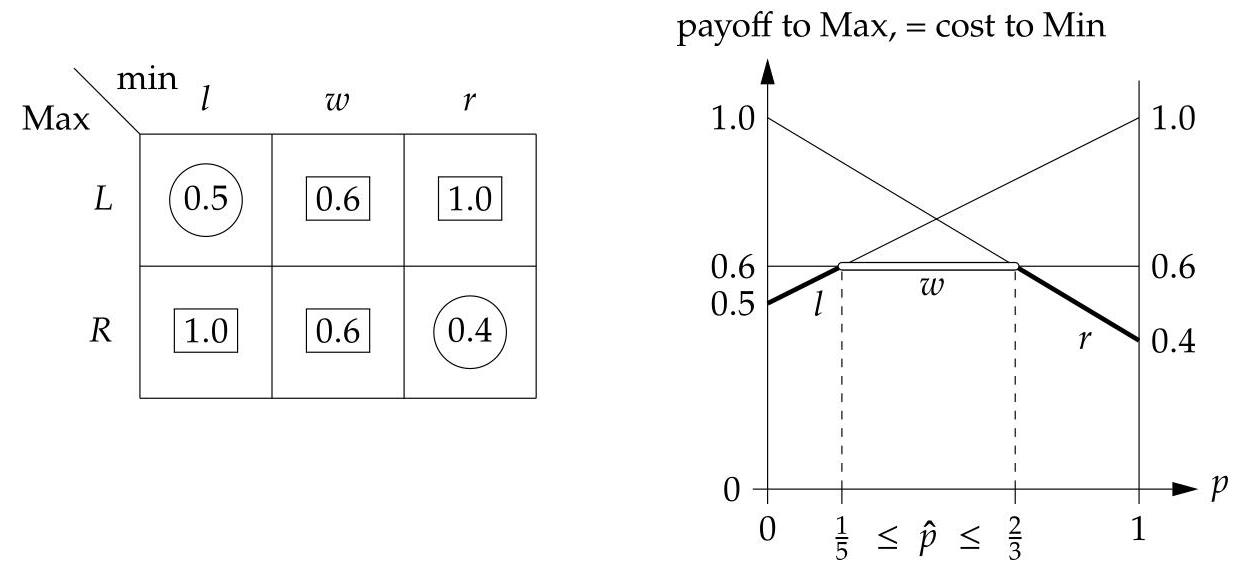
\includegraphics[width=0.8\linewidth]{images/ch08-fig03.jpg}
    \caption{ 当列玩家选择 \(w\) 时，罚球博弈的得分概率相同，均为$0.6$。此时博弈是退化的，极大极小策略 \(\left( {1 - \widehat{p},\widehat{p}}\right)\) 不是唯一的， \(\widehat{p} \in  \left\lbrack  {\frac{1}{5},\frac{2}{3}}\right\rbrack\)。}
    \label{fig:8.3}
\end{figure}

\(\Rightarrow\) 练习~\ref{exer:8.1}给出点球博弈的一个变体：射手的进球概率更高，并且在(b)部分还多了第三种策略 \(M\)，即向中间射门。

\section{极大极小和极小极大策略}\label{sec:8.3}

零和博弈引入的一个重要概念是极大极小策略。原则上，这个概念可以用于任何博弈；这里我们只讨论两人博弈。极大极小策略是从玩家自身收益出发定义的，也依赖于玩家可选择的策略集。下面的定义使用一般的非空策略集 \(X\) 和 \(Y\)；它们通常是\eqref{eq:6.6}中的混合策略集，但并不一定必须如此。极小极大策略则是从另一名玩家的角度得到的对应概念。

\begin{definition}[极大极小策略，极小极大策略]\label{def:8.1}
考虑一个双人博弈，玩家I的策略集为 \(X\) ，玩家II的策略集为 \(Y\) ，当玩家I选择 \(x \in  X\) 且玩家II选择 \(y \in  Y\) 时，玩家I的收益为 \(a\left( {x,y}\right)\) 。玩家I的极大极小策略 \(\widehat{x} \in  X\) 满足

\begin{equation}\label{eq:8.1}
    \min_{{y \in  Y}}a\left( {\widehat{x},y}\right)  =\max_{{x \in  X}}\min_{{y \in  Y}}a\left( {x,y}\right)
\end{equation}

假设这些最小值和最大值存在，这就定义了玩家I的极大极小收益。玩家II的极小极大策略 \(\widehat{y} \in  Y\) 满足

\begin{equation}\label{eq:8.2}
    \max_{{x \in  X}}a\left( {x,\widehat{y}}\right)  = \min_{{y \in  Y}}\max_{{x \in  X}}a\left( {x,y}\right)
\end{equation}
这就定义了玩家I的极小极大收益。
\end{definition}


先看一个有限博弈，例如图~\ref{fig:8.2}右上方的博弈，其中行玩家 \(I\) 的收益矩阵 \(A\) 是 \(2 \times  3\) 矩阵。若定义~\ref{def:8.1}中的策略集取为 \(X = \{ L,R\}\) 和 \(Y = \{ l,w,r\}\)，则式\eqref{eq:8.1}和\eqref{eq:8.2}中的最小值和最大值显然存在。由于玩家I此时不能随机化，他只能比较选择 \(L\) 时能保证的最低收益0.5，以及选择 \(R\) 时能保证的最低收益0.4，两者在图中用圆圈标出。因此他的极大极小策略是 \(L\)，极大极小收益为0.5。对极小极大策略而言，列玩家II要比较玩家I面对 \(l,w,r\) 时分别能取得的最大收益，即1.0、0.7和1.0，图中用方框标出。因此极小极大策略是 \(w\)，极小极大收益为0.7。在这个纯策略版本中，极大极小收益和极小极大收益并不相等。

通常我们考虑有限博弈的混合扩展(mixed extension)。此时 \(X\) 和 \(Y\) 是混合策略集，定义~\ref{def:8.1}中玩家I的收益为 \(a\left( {x,y}\right)  = {x}^{\top }{Ay}\)。根据图~\ref{fig:8.2}中的门柱图，玩家 \(\mathrm{I}\) 的混合极大极小策略为 \(\widehat{x} = \left( {\frac{2}{3},\frac{1}{3}}\right)\)，极大极小收益为 \(\frac{2}{3}\)。我们马上会看到，玩家II的极小极大策略正是她的均衡策略 \(\left( {\frac{1}{6},\frac{5}{6},0}\right)\)，而玩家I的极小极大收益同样为 \(\frac{2}{3}\)。

极大极小策略的基本想法是：无论对手采取什么行动，它都能为玩家保证一个尽可能高的期望收益。因此，极大极小策略有时也称为“安全策略”(security strategy)。若玩家I选择 \(x\)，他的最坏情况收益是 \(\min_{{y \in  Y}}a\left( {x,y}\right)\)。式\eqref{eq:8.1}中的极大极小策略 \(\widehat{x}\) 就是使这个最坏情况收益最大化的策略，并由此给出玩家I的极大极小收益。在一般收益博弈中，玩家II未必真的想选择使 \(a\left( {x,y}\right)\) 最小的策略 \(y\)。但在零和博弈中，这个 \(y\) 正是玩家II对 \(x\) 的最优反应，所以玩家I应当预期这种反应。

式\eqref{eq:8.2}中的极小极大策略 \(\widehat{y}\) 则从玩家II的角度出发。玩家II假定玩家I会对 \(\widehat{y}\) 作出最优反应，从而取得 \(\max_{{x \in  X}}a\left( {x,\widehat{y}}\right)\)；她选择 \(\widehat{y}\)，就是为了使这个数尽可能小。在一般收益博弈中，这等于假设玩家II一心惩罚玩家I，从她自身收益的安全性来看未必合理。

但在零和博弈中，极小极大策略只不过是最小化者一侧的极大极小策略。具体说，设零和博弈为(A, B)，其中 \(B =  - A\)。对于 \(a\left( {x,y}\right)  = {x}^{\top }{Ay}\)，极小极大策略 \(\widehat{y}\) 满足式\eqref{eq:8.2}，也等价于

\[
\min_{{x \in  X}}{x}^{\top }B\widehat{y} =\max_{{y \in  Y}}\min_{{x \in  X}}{x}^{\top }{By}
\]

因此， \(\widehat{y}\) 正是按玩家II的收益矩阵 \(B\) 得到的极大极小策略。也就是说，在零和博弈中，极小极大策略不是一个真正不同的概念；它只是用玩家II的成本矩阵 \(A\) 来表达玩家II的偏好，而这个矩阵同时也是玩家I的收益矩阵，并由它定义整个矩阵博弈。

定义~\ref{def:8.1}假设相关的最小值和最大值存在。若 \(X\) 和 \(Y\) 是紧集，且 \(a\left( {x,y}\right)\) 关于 \(x\) 和 \(y\) 连续，这个假设就成立。矩阵博弈 \(A\) 的混合策略集正满足这些条件，此时 \(a\left( {x,y}\right)  = {x}^{\top }{Ay}\)。下面的命题说明，在 \(\max_{{x \in  X}}\min_{{y \in  Y}}{x}^{\top }{Ay}\) 中，内层最小值其实已经能由某个纯策略 \(j\) 达到，而不必考虑所有混合策略 \(y\in Y\)；图~\ref{fig:8.2}中的下包络正是这样得到的。类似地，在 \(\min_{{y \in  Y}}\max_{{x \in  X}}{x}^{\top }{Ay}\) 中，内层最大值也可由某个纯策略 \(i\) 达到。


\begin{proposition}\label{prop:8.2}
     对于一个 \(m \times  n\) 矩阵博弈 \(A\) 和 \(x \in  X\) ，
\begin{equation}\label{eq:8.3}
    \min_{{y \in  Y}}{x}^{\top }{Ay} = \min \left\{  {{\left( {x}^{\top }A\right) }_{j} \mid  1 \leq  j \leq  n}\right\}.
\end{equation}


对于 \(y \in  Y\) ，

\begin{equation}\label{eq:8.4}
    \max_{{x \in  X}}{x}^{\top }{Ay} = \max \left\{  {{\left( Ay\right) }_{i} \mid  1 \leq  i \leq  m}\right\}.
\end{equation}


此外，存在一个极大极小策略 \(\widehat{x} \in  X\) 和一个极小极大策略 \(\widehat{y} \in  Y\) 。
\end{proposition}
\begin{proof}
设 \(y \in  Y\) 。最优反应条件\eqref{eq:6.10}表明，对 \(y\) 的最优反应(best response)可以在行玩家的纯策略 \(i\) 中找到，这意味着式\eqref{eq:8.4}成立。类似地，条件\eqref{eq:8.3}也成立。

式\eqref{eq:8.3}的右边是有限项 \({\left( {x}^{\top }A\right) }_{j}\) 的最小值，且关于 \(x\) 连续。因此，相等的左边 \(\min_{{y \in  Y}}{x}^{\top }{Ay}\) 关于 \(x\) 也连续，并且在紧集 \(X\) 上的某个 \(\widehat{x}\) 处取得最大值。那么 \(\widehat{x}\) 定义了一个极大极小策略。类似地，存在一个极小极大策略 \(\widehat{y}\) 。
\end{proof}

极大极小收益和极小极大成本都是在期望意义下可以保证的数，因此前者不可能高于后者。设 \(\widehat{x}\) 和 \(\widehat{y}\) 分别是定义~\ref{def:8.1}中的极大极小策略和极小极大策略，则有

\begin{equation}\label{eq:8.5}
\begin{aligned}
\max_{{x \in  X}}\min_{{y \in  Y}}a\left( {x,y}\right)  &= \min_{{y \in  Y}}a\left( {\widehat{x},y}\right)\\
&\leq  a\left( {\widehat{x},\widehat{y}}\right)\\
&\leq \max_{{x \in  X}}a\left( {x,\widehat{y}}\right)  = \min_{{y \in  Y}}\max_{{x \in  X}}a\left( {x,y}\right).
\end{aligned}
\end{equation}
这给出了几乎显然的收益不等式“极大极小 \(\leq\) 极小极大”。只要 \(X\) 和 \(Y\) 非空且有关的最小值、最大值存在，这个不等式就成立。前面已经看到，当 \(X\) 和 \(Y\) 是纯策略集时，不等式可能是严格的。

如果 \(X\) 和 \(Y\) 是混合策略集，且 \(a\left( {x,y}\right)  = {x}^{\top }{Ay}\)，冯·诺伊曼(1928)著名的极小极大定理指出，上述不等式取等号，也就是“极大极小 = 极小极大”。下面的命题说明，这个等式等价于 \(\left( {\widehat{x},\widehat{y}}\right)\) 是该博弈的均衡。

\begin{proposition}\label{prop:8.3}考虑一个 \(m \times  n\) 矩阵博弈 \(A\) ，其混合策略集为 \(X\) 和 \(Y\) ，如\eqref{eq:6.6}所示，并且设 \(\left( {{x}^{ * },{y}^{ * }}\right)  \in  X \times  Y\) 。那么以下表述等价:

(a) \(\left( {{x}^{ * },{y}^{ * }}\right)\) 是$(A, -A)$的一个均衡；

(b) \({x}^{ * }\) 是一个极大极小策略， \({y}^{ * }\) 是一个极小极大策略，并且

\begin{equation}\label{eq:8.6}
\max_{{x \in  X}}\min_{{y \in  Y}}{x}^{\top }{Ay} = \min_{{y \in  Y}}\max_{{x \in  X}}{x}^{\top }{Ay}.
\end{equation}
\end{proposition}
\begin{proof}
 假设(b)成立。考虑如\eqref{eq:8.1}所示的极大极小策略 \(\widehat{x}\) 和如\eqref{eq:8.2}所示的极小极大策略 \(\widehat{y}\) 。那么\eqref{eq:8.6}意味着

\begin{align*}
{\widehat{x}}^{\top }A\widehat{y} &\geq  \min_{{y \in  Y}}{\widehat{x}}^{\top }{Ay}\\
&=\max_{{x \in  X}}\min_{{y \in  Y}}{x}^{\top }{Ay}\\
&=\max_{{x \in  X}}{x}^{\top }A\widehat{y} \geq  {\widehat{x}}^{\top }A\widehat{y}
\end{align*}


因此所有这些不等式都取等号。所以，

\begin{equation}\label{eq:8.7}
\max_{{x \in  X}}{x}^{\top }A\widehat{y} = {\widehat{x}}^{\top }A\widehat{y} = \min_{{y \in  Y}}{\widehat{x}}^{\top }{Ay}
\end{equation}

这表明 \(\left( {\widehat{x},\widehat{y}}\right)\) 是一个均衡，因为\eqref{eq:8.7}等价于

\begin{equation}\label{eq:8.8}
{x}^{\top }A\widehat{y} \leq  {\widehat{x}}^{\top }A\widehat{y} \leq  {\widehat{x}}^{\top }{Ay}\;\text{ for all }x \in  X,y \in  Y
\end{equation}

其中\eqref{eq:8.8}中的左不等式表明 \(\widehat{x}\) 是对 \(\widehat{y}\) 的最优反应，右不等式表明 \(\widehat{y}\) 是对 \(\widehat{x}\) 的最优反应。这证明了(a)。

反之，假设(a)成立，即如\eqref{eq:8.7}所示，

\[
\max_{{x \in  X}}{x}^{\top }A{y}^{ * } = {x}^{*\top }A{y}^{ * } = \min_{{y \in  Y}}{x}^{*\top }{Ay}.
\]

利用\eqref{eq:8.5}，这意味着

\begin{align*}
{x}^{*\top }A{y}^{*} &= \min_{{y \in  Y}}{x}^{*\top }{Ay}\\
&\leq \max_{{x \in  X}}\min_{{y \in  Y}}{x}^{\top }{Ay}\\
&\leq  \min_{{y \in  Y}}\max_{{x \in  X}}{x}^{\top }{Ay}\\
&\leq \max_{{x \in  X}}{x}^{\top }A{y}^{ * } = {x}^{*\top }A{y}^*
\end{align*}

因此我们同样处处取等号，这表明 \({x}^{ * }\) 是一个极大极小策略， \({y}^{ * }\) 是一个极小极大策略，并且\eqref{eq:8.6}成立，这证明了(b)。
\end{proof}


因此，极小极大定理也可以看作纳什(1951)定理~\ref{theo:6.5}的一个推论。

\begin{theorem}[冯·诺伊曼的极小极大定理，1928]\label{theo:8.4}在一个矩阵博弈中，最大化者即行玩家 \(I\) 的收益矩阵为 \(A\)，玩家I和玩家II的混合策略集分别为 \(X\) 和 \(Y\)，则
\begin{equation}\label{eq:8.9}
\max_{{x \in  X}}\min_{{y \in  Y}}{x}^{\top }{Ay} = v = \min_{{y \in  Y}}\max_{{x \in  X}}{x}^{\top }{Ay}
\end{equation}

其中 \(v\) 是玩家I唯一的极大极小收益，也是玩家II唯一的极小极大成本，称为博弈的值。
\end{theorem}
纳什定理通常借助布劳威尔不动点定理证明，而该定理本身较为复杂。下一节将给出极小极大定理~\ref{theo:8.4}的一个简短且自包含的证明。

两人零和博弈的均衡策略具有一些非常好的性质，而这些性质在一般收益博弈中通常不成立：

\begin{itemize}
\item 玩家的均衡收益唯一确定，称为博弈的值；在\eqref{eq:8.9}中，它就是最大化者的收益 \(v\)，也是最小化者的成本。
\item 均衡策略与最大化者的极大极小策略、最小化者的极小极大策略一致。因此，它不依赖于对方实际如何行动。由于这个原因，它也称为玩家的最优策略。
\end{itemize}

“最优策略”默认玩家会以最有利于自己的方式行动。它通常相当保守：面对对手的许多不同应对，它都给出相同的期望效用。例如，对称零和博弈的值必然为零(见练习~\ref{exer:8.3}(c))。因此，最大化者的最优策略保证他在面对对手任意纯策略时，至少得到零收益，即使对手并没有采用最优策略。这样做可能无法利用对手的失误，但它绝不会伤害采用最优策略的玩家。

由于最优策略不依赖于对方策略，还可以得到：

\begin{itemize}
\item 在零和博弈中，均衡策略可以交换：如果$(x, y)$和 \(\left( {\bar{x},\bar{y}}\right)\) 是同一零和博弈的两个均衡，那么 \(\left( {\bar{x},y}\right)\) 和 \(\left( {x,\bar{y}}\right)\) 也都是均衡。
\item 如命题~\ref{prop:8.3}所述，零和博弈中的均衡策略就是极大极小策略(或极小极大策略)。例如，如果某个零和博弈存在一个均衡，并且其中一方有唯一的纯最优反应，那么这个纯策略也是最大化者唯一的极大极小策略，或最小化者唯一的极小极大策略。理由是，如果比如极小极大策略不唯一，那么它在任何均衡中也不会唯一。图~\ref{fig:8.3}中的博弈正说明这一点：极大极小策略为 \(\left( {1 - \widehat{p},\widehat{p}}\right)\)，其中 \(p \in  \left\lbrack  {\frac{1}{5},\frac{2}{3}}\right\rbrack\)；对该区间内部任意 \(\widehat{p}\)，例如 \(\widehat{p} = \frac{1}{2}\)，玩家II的唯一最优反应都是纯策略 \(w\)，因此 \(w\) 也是玩家II唯一的均衡策略和极小极大策略。
\end{itemize}

第~\ref{sec:8.5} 节还会讨论两个性质：最优策略集是凸的(命题~\ref{prop:8.6})；移除弱被占优策略(weakly dominated strategy)不会改变博弈值(命题~\ref{prop:8.7})。不过，后一种移除可能会改变最优策略集本身。

\section{ 极小极大定理的简短证明}\label{sec:8.4}

根据命题~\ref{prop:8.3}，冯·诺伊曼(1928)的极小极大定理~\ref{theo:8.4}可以看作纳什有限博弈均衡存在性定理~\ref{theo:6.5}的一个特例。不过，冯·诺伊曼的结果早于纳什定理，而且可以独立证明。下面给出一个特别简洁的归纳证明。

\begin{theorem}\label{theo:8.5}对于一个 \(m \times  n\) 矩阵博弈 \(A\) ，其混合策略集为\eqref{eq:6.6}中的 \(X\) 和 \(Y\) ，存在 \(x \in  X,y \in  Y\) 和 \(v \in  \mathbb{R}\) 使得

\[
{Ay} \leq  \boldsymbol{1}v,\;{x}^{\top }A \geq  v{ \boldsymbol{1}}^{\top }.
\]

那么 \(v\) 是该博弈的唯一价值，并且\eqref{eq:8.9}成立， \(x\) 和 \(y\) 是玩家的最优策略。
\end{theorem}
\begin{proof}考虑两个优化问题(其中 \(v,u \in  \mathbb{R}\) )

\begin{equation}\label{eq:8.10}
\mathop{\operatorname{minimize}}\limits_{{y,v}}v\;\text{ subject to }{Ay} \leq  \boldsymbol{1}v,\;y \in  Y.
\end{equation}

以及

\begin{equation}\label{eq:8.11}
\mathop{\operatorname{maximize}}\limits_{{x,u}}u\text{ subject to }{x}^{\top }A \geq  u{\boldsymbol{1}}^{\top },\;x \in  X.
\end{equation}

不等式 \({Ay} \leq  \boldsymbol{1}{v}\) 的含义是：玩家II采用策略 \(y\) 时，无论落在哪一行，他支付给玩家I的数额都不超过 \(v\)。类似地，\({x}^{\top }A \geq  u{\boldsymbol{1}}^{\top }\) 表示玩家I采用策略 \(x\) 时，无论玩家II选择哪一列，他至少能得到 \(u\)。

设 \(y,v\) 是 \eqref{eq:8.10} 的最优解。那么 \(m\) 个不等式 \({Ay} \leq  \boldsymbol{1}v\) 中至少有一个取等号，因为如果所有不等式都是严格不等式，那么 \(v\) 可以进一步减小。因此， \(v\) 是 \({Ay}\) 的最大元素 \({\left( Ay\right) }_{i}\) (就像对 \(y\) 的任何纯最优反应 \(i\) 一样)，根据 \eqref{eq:8.4} 满足

\[
v =\max_{{1 \leq  i \leq  m}}{\left( Ay\right) }_{i} =\max_{{y \in  Y}}{x}^{\top }{Ay}
\]

并且 \eqref{eq:8.10} 中 \(y\) 的最优选择是一个极小极大策略。类似地，对于 \eqref{eq:8.11} 中的最优对 \(x,u\) ，根据 \eqref{eq:8.3} 我们有

\[
u = \min_{{1 \leq  j \leq  n}}{\left( {x}^{\top }A\right) }_{j} = \min_{{y \in  Y}}{x}^{\top }{Ay}
\]

其中 \(x\) 是一个极大极小策略。

考虑问题 \eqref{eq:8.10} 和 \eqref{eq:8.11} 的可行(不一定是最优)解 \(y,v,x,u\) ，即

\begin{equation}\label{eq:8.12}
{Ay} \leq  \mathbf{1}v,\;y \in  Y,\;{x}^{\top }A \geq  u{\mathbf{1}}^{\top },\;x \in  X.
\end{equation}

那么

\begin{equation}\label{eq:8.13}
u = u{\mathbf{1}}^{\top }y \leq  {x}^{\top }{Ay} \leq  {x}^{\top }\mathbf{1}v = v.
\end{equation}

这说明 \eqref{eq:8.10} 和 \eqref{eq:8.11} 的目标函数都有界；而且在不改变最优值的情况下，可以把搜索范围限制在非空紧集上。具体说，若某个 \(\bar{y},\bar{v},\bar{x},\bar{u}\) 满足 \eqref{eq:8.12}，则只需考虑 \(\left( {y,v}\right)  \in  Y \times  \left\lbrack  {\bar{u},\bar{v}}\right\rbrack\) 和 \(\left( {x,u}\right)  \in  X \times  \left\lbrack  {\bar{u},\bar{v}}\right\rbrack\)。因此，\eqref{eq:8.10} 和 \eqref{eq:8.11} 的最优值 \(v\) 和 \(u\) 存在，且各自唯一。剩下要证明的是 \(u = v\)，这正是“极大极小 = 极小极大”，也就是 \eqref{eq:8.9}。

我们通过对 \(m + n\) 进行归纳来证明这个结论。对于 \(m + n = 2\) 来说这是显然的。考虑任意维度 \(m \times  n\) 的矩阵 \(A\) ，并设 \(y,v\) 和 \(x,u\) 分别是 \eqref{eq:8.10} 和 \eqref{eq:8.11} 的最优解，它们是可行的，即 \eqref{eq:8.12} 成立。如果 \eqref{eq:8.12} 中的所有不等式都取等号，即 \({Ay} = \mathbf{1}v\) 和 \(u{\mathbf{1}}^{\top } = {x}^{\top }A\) ，那么 \eqref{eq:8.13} 也取等号，并且如所声称的 \(u = v\) 。因此，我们可以假设 \({Ay} \leq  \mathbf{1}v\) 中至少有一个不等式是严格的(或者在 \({x}^{\top }A \geq  u{\mathbf{1}}^{\top }\) 中，同样的推理适用)。假设这是第 \(k\) 行，即，对于矩阵 \(A\) 的元素 \({a}_{ij}\) ，

\begin{equation}\label{eq:8.14}
\sum\limits_{{j = 1}}^{n}{a}_{kj}{y}_{j} < v
\end{equation}

设 \(\bar{A}\) 是去掉 \(k\) 行后的矩阵 \(A\) (显然 \(m > 1\) )。设 \(\bar{y},\bar{v}\) 是用 \(\bar{A}\) 代替 \(A\) 时 \eqref{eq:8.10} 的最优解，即

\begin{equation}\label{eq:8.15}
\mathop{\operatorname{minimize}}\limits_{{\bar{y},\bar{v}}}\bar{v}\text{ subject to }\bar{A}\bar{y} \leq  \mathbf{1}\bar{v},\;\bar{y} \in  Y.
\end{equation}

用 \(\bar{A}\) 代替 \(A\) 时，与 \eqref{eq:8.11} 对应的最大化问题可以写成

\begin{equation}\label{eq:8.16}
\mathop{\operatorname{maximize}}\limits_{{\bar{x},\bar{u}}}\bar{u}\text{ subject to }{\bar{x}}^{\top }A \geq  \bar{u}{\mathbf{1}}^{\top },\;\bar{x} \in  X,\;{\bar{x}}_{k} = 0.
\end{equation}

设 \(\bar{x},\bar{u}\) 是 \eqref{eq:8.16} 的最优解。那么

\begin{equation}\label{eq:8.17}
\bar{u} \leq  u,\;\bar{v} \leq  v
\end{equation}

因为 \(\bar{x},\bar{u}\) 是 \eqref{eq:8.11} 的可行解(所以对于 \eqref{eq:8.11} 中的最大值 \(u\) 有 \(\bar{u} \leq  u\) )，并且因为 \(y,v\) 是 \eqref{eq:8.15} 的可行解。直观地说，\eqref{eq:8.17} 成立是因为博弈 \(\bar{A}\) 对玩家 II 至少和博弈 \(A\) 一样有利。根据归纳假设， \(\bar{u} = \bar{v}\) 。

我们声称(这是关键点) \(\bar{v} = v\) 。即，如果 \(\bar{v} < v\) ，设 \(\varepsilon  \in  (0,1\rbrack\) ，那么 \(v\left( {1 - \varepsilon }\right)  + \bar{v}\varepsilon  = v - \varepsilon \left( {v - \bar{v}}\right)  < v\) 。考虑策略 \({y}^{\prime } = y\left( {1 - \varepsilon }\right)  + \bar{y}\varepsilon\) ，它属于 \(Y\) ，因为 \(Y\) 是凸集。由于 \(\bar{A}y \leq  \mathbf{1}v\) 且根据 \eqref{eq:8.15}， \({y}^{\prime }\) 满足

\[
\bar{A}{y}^{\prime } = \bar{A}\left( {y\left( {1 - \varepsilon }\right)  + \bar{y}\varepsilon }\right)  \leq  \mathbf{1}\left( {v\left( {1 - \varepsilon }\right)  + \bar{v}\varepsilon }\right)  < \mathbf{1}v.
\]

类似地，\eqref{eq:8.14} 意味着对于足够小的 \(\varepsilon\)

\[
\sum\limits_{{j = 1}}^{n}{a}_{kj}{y}_{j}^{\prime } = \sum\limits_{{j = 1}}^{n}{a}_{kj}{y}_{j} + \varepsilon \sum\limits_{{j = 1}}^{n}{a}_{kj}\left( {{\bar{y}}_{j} - {y}_{j}}\right)  < v
\]

这意味着存在 \({y}^{\prime } \in  Y\) 和 \({v}^{\prime } < v\) 使得 \(A{y}^{\prime } \leq  \mathbf{1}{v}^{\prime }\) ，这与 \eqref{eq:8.10} 中 \(v\) 的极小性相矛盾。这表明 \(v = \bar{v}\) 。

结合 \eqref{eq:8.17} 可得 \(\bar{u} \leq  u \leq  v = \bar{v} = \bar{u}\) ，因此 \(u = v\) ，这正是我们要证明的。
\end{proof}

这个归纳证明的思路可以概括如下：如果两名玩家的最优策略已经使所有相关行列的收益分别等于 \(v\) 和 \(u\)，那么立刻得到 \(u = v\)。否则，必要时交换两名玩家的角色，至少有一行的收益严格低于 \(v\)。行玩家在最优策略中不会使用这一行，于是可以把它从博弈中删去，并对较小的博弈应用归纳假设。

优化问题 \eqref{eq:8.10} 是线性规划(linear programming)的一个特例：在线性等式和不等式约束下，优化一个线性函数。这里的变量是 \(\left( {y,v}\right)  \in  {\mathbb{R}}^{n} \times  \mathbb{R}\)，目标函数是需要最小化的 \(v\)，约束为 \({Ay} - \mathbf{1}v \leq  \mathbf{0},y \geq  \mathbf{0},{\mathbf{1}}^{\top }y = 1\)。最大化问题 \eqref{eq:8.11} 则是 \eqref{eq:8.10} 的对偶线性规划。它使用同一组数据，但从转置方向处理矩阵，并交换右端项与目标函数的角色。这里不展开精确定义，相关参考见第~\ref{sec:8.6} 节。

不等式 \eqref{eq:8.13} 是线性规划弱对偶性的一个特殊情形，和 \eqref{eq:8.5} 一样几乎显然。线性规划的强对偶定理进一步说明，如果原问题和对偶问题都可行，那么它们的最优值不仅互为上下界，而且实际相等。极小极大定理便可由此立即推出。

线性规划对偶是一套优美而实用的理论，定理~\ref{theo:8.5} 的证明可以作为一个很好的入口。另一方面，现代线性规划算法已经能够处理几十万甚至上百万个变量和约束，也可以用来计算零和博弈的最优策略。

\section{零和博弈进一步说明}\label{sec:8.5}

极大极小策略和极大极小收益只取决于玩家自己的收益。因此，即使在并非零和的一般收益博弈中，甚至在 \(N\) 人博弈中，也可以定义这个概念。此时，极大极小策略体现的是一种相当悲观的看法：玩家 I 选择策略 \(\widehat{x}\)，好像其他对手都只想伤害他一样，并在这种最坏情况下最大化自己的收益。在零和博弈中，这种设想正好符合对手的目标。式\eqref{eq:8.2}中的极小极大策略也可以为一般博弈定义，但解释不同：对手选择策略 \(\widehat{y}\) 来惩罚玩家 \(\mathrm{I}\)，而玩家 \(\mathrm{I}\) 随后可以选择 \(x\) 来防御。极小极大收益就是这种方式能够施加给玩家 I 的最大惩罚。在多于两个玩家的博弈中，这也有意义：其他玩家可以约定一个部分混合策略组合 \(\widehat{y}\)，以最大限度地惩罚玩家 I。这类“惩罚策略”常用于重复博弈中维持某些均衡，本书不展开讨论。

本章只考虑零和博弈中的极大极小策略和极小极大策略。在零和博弈中，这两个概念本质相同，并且建立在一个合理预期之上：对手会采取对自己最有利、也就是对你最不利的反应，而你需要对此作出最优应对。

下面对零和博弈中最大化者的极大极小策略，以及最小化者的极小极大策略，再作几点观察。

\begin{proposition}\label{prop:8.6}
    在零和博弈中，每个参与者的最优策略集是凸集。
\end{proposition}
\begin{proof}
    这可由命题~\ref{prop:8.3}和命题~\ref{prop:6.9}推出。
\end{proof} 

在零和博弈中，忽略弱被占优策略不会改变博弈的值。
\begin{proposition}\label{prop:8.7}
    考虑两个矩阵博弈 \(A\) 和 \({A}^{\prime }\) ，其中 \({A}^{\prime }\) 是通过移除其中一个参与者的弱被占优策略从 \(A\) 得到的。那么 \({A}^{\prime }\) 的任何(混合)均衡都是 \(A\) 的均衡，并且 \(A\) 和 \({A}^{\prime }\) 具有相同的博弈值。
\end{proposition}
\begin{proof}
取 \({A}^{\prime }\) 的任意一个混合均衡，把它自然看作 \(A\) 中的一个混合策略对。根据最优反应条件，只要不存在向某个纯策略的有利偏离，它就是 \(A\) 中的均衡。在 \({A}^{\prime }\) 中不可行的唯一潜在偏离，是转向被删去的弱被占优策略；但如果转向这个策略是有利的，那么转向占优它的策略同样有利，而后者在 \({A}^{\prime }\) 中仍然可行。因此， \({A}^{\prime }\) 的均衡也是 \(A\) 的均衡。命题~\ref{prop:3.3}(a)给出了类似结论，不过那里讨论的是纯均衡。由命题~\ref{prop:8.3}可知，零和博弈的均衡收益就是博弈值，所以 \(A\) 和 \({A}^{\prime }\) 的博弈值相同。
\end{proof}


下面这个博弈的纯最优反应标在右侧，它有两个纯均衡 $(T, l)$和 $(T, r)$。因此， \(l\) 和 \(r\) 的任意凸组合，也就是最小化者的任意混合策略，都是极小极大策略。唯一的极大极小策略是 \(T\)，因为它是对 \(l\) 的唯一最优反应。该博弈的值为1。若从博弈中删去弱被占优策略 \(B\) 和 \(r\)，博弈值仍为1；但 \(r\) 也因此不再可能作为极小极大策略出现。所以，如果我们只关心零和博弈的值，通常可以移除弱被占优策略并反复这样做；但最优策略集可能会因此缩小。


\begin{center}
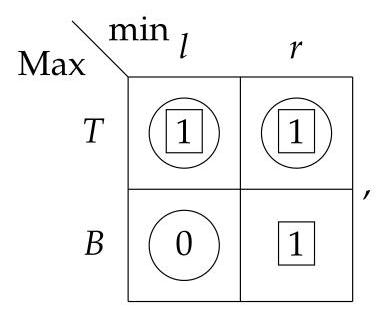
\includegraphics[width=0.4\textwidth]{images/ch08-fig04.jpg}
\end{center}
\hspace*{3em} 

\section{延伸阅读}\label{sec:8.6}

极小极大定理的历史可参见冯·诺伊曼和弗雷歇(1953)的讨论。在《计量经济学》同一期较早的一篇文章中，弗雷歇说明了数学家埃米尔·博雷尔如何首先提出在博弈中使用主动随机化(即混合策略)，并把对称零和博弈中的这一结论作为开放问题提出。冯·诺伊曼(1928)最早证明了该定理；当时他并不知道博雷尔的论文和问题。此后，该定理的证明被大大简化。

定理~\ref{theo:8.5}的简短归纳证明归功于卢米斯(1946)。卢米斯给出的表述更一般，这里只把它用于零和博弈。这个证明与欧文(1967)的证明非常接近；欧文只消除一个严格不等式来应用归纳假设，而卢米斯(1946)则消除所有这类不等式。

极小极大定理(minimax theorem)的一个几何证明(冯·诺伊曼和摩根斯坦在1947年的著作中也使用了该证明)基于分离超平面(separating hyperplane)定理(见推论~\ref{cor:7.16}和图~\ref{fig:7.13})。该定理适用于以下情况，在此情况下它被称为法卡斯定理(Farkas’s Lemma):设 \(A \in  {\mathbb{R}}^{d \times  n}\) 且 \(x \in  {\mathbb{R}}^{d}\) ，并假设 \(x \notin  D = \left\{  {{Ay} \mid  y \in  {\mathbb{R}}^{n},y \geq  \mathbf{0}}\right\}\) 。该引理表明，存在某个 \(v \in  {\mathbb{R}}^{d}\) 使得 \({v}^{\top }A \geq  {\mathbf{0}}^{\top }\) 且 \({v}^{\top }x < 0\) 。集合 \(D\) 是矩阵 \(A\) 各列的非负线性组合构成的“凸锥”，如果向量 \(x\) 不在该锥内，那么存在一个以 \(v\) 为法向量(normal vector)的“分离超平面”，使得矩阵 \(A\) 的所有列都在超平面 \(\left( {{v}^{\top }A \geq  {\mathbf{0}}^{\top }}\right)\) 的一侧，而向量 \(x\) 严格位于另一侧 \(\left( {{v}^{\top }x < 0}\right)\) 。如果能证明(这是唯一缺失的部分) \(D\) 是闭集，那么这就是推论~\ref{cor:7.16}的一个结果。因为 \(D\) 是闭集，所以可以选择 \(c\) 作为 \(D\) 中距离 \(x\) 最近的点，并令 \(v = c - x\) (根据推论~\ref{cor:7.16}后的描述，它与 \(v\) 符号相反)。那么 \(D \subseteq  \left\{  {z \in  {\mathbb{R}}^{d} \mid  {v}^{\top }z \geq  \alpha }\right\}\) ，其中 \(\alpha  = {v}^{\top }c =  - {\left( x - c\right) }^{\top }c = 0\) ，因为如果还不满足 \(c = \mathbf{0}\) ，那么类似于引理~\ref{lem:7.17}可以看出， \(x - c\) 与射线 \(\{ {c\beta } \mid  \beta  \geq  0\}\) 正交(orthogonal)，而该射线是 \(D\) 的一个子集；这也意味着 \({v}^{\top }\left( {x - c}\right)  =  - \parallel v{\parallel }^{2} < 0\) ，从而 \({v}^{\top }x < {v}^{\top }c = 0\) 。

线性规划的强对偶定理，进而极小极大定理，可以通过对法卡斯定理进行一些进一步的代数运算来证明(见Gale，1960，第78页及以后)。关于线性规划的经典著作是Dantzig(1963)。通俗易懂的介绍有Chvátal(1983)，特别是从几何角度介绍的有Matoušek和Gärtner(2007)。一本具有出色历史参考文献的学术著作是Schrijver(1986)。从线性规划对偶(linear programming duality)很容易得到极小极大定理；相反的方向已由Adler(2013)进行了研究。

\section{第8章习题}\label{sec:8.7}
\begin{exercise}\label{exer:8.1}
 考虑下面的点球博弈。行玩家是射手，可选择 \(L\) (向左射门)或 \(R\) (向右射门)；列玩家是守门员，可选择 \(l\) (向左扑)、 \(w\) (等待后再扑)或 \(r\) (向右扑)。矩阵中的数字表示进球概率。行玩家希望最大化这个概率，列玩家希望最小化这个概率。
\begin{center}
\adjustbox{width=0.5\textwidth}{
\begin{tabular}{|c|c|c|c|}
\hline
\multirow{3}{*}{最大值 \(L\)  \(R\)} & 最小值 \(l\) & \(w\) & r \\
\cline{2-4}
 & 0.6 & 0.7 & 1.0 \\
\cline{2-4}
 & 1.0 & 0.8 & 0.7 \\
\cline{1-4}
\hline
\end{tabular}
}
\end{center}

(a) 找出该博弈在混合策略(包括纯策略)下的所有均衡(equilibrium)及其均衡收益。为什么收益是唯一的？

(b) 现在假设玩家I有一个额外的策略 \(M\) (向中间射门)，使得收益矩阵为

\begin{center}
\adjustbox{width=0.5\textwidth}{
\begin{tabular}{|c|c|c|c|}
\hline
Max & \({\text{min }}l\) & \(w\) & \(r\) \\
\cline{1-4}
\multirow{3}{*}{\(L\)  \(R\)  \(M\)} & 0.6 & 0.7 & 1.0 \\
\cline{2-4}
 & 1.0 & 0.8 & 0.7 \\
\cline{2-4}
 & 1.0 & 0.0 & 1.0 \\
\cline{1-4}
\hline
\end{tabular}
}
\end{center}

找出该博弈的一个均衡以及均衡收益。[提示:(a) 部分的结果会有用。]
\end{exercise}

\begin{exercise}\label{exer:8.2}
(a) 考虑一个零和博弈，其中每个纯策略的最优反应是唯一的。假设最上面一行和最左边一列确定了该博弈的一个纯策略均衡。证明这个均衡可以通过迭代消除严格被占优策略来找到。[提示:首先考虑 \(n = 2\) 的情况。]

(b) 如果某些纯策略有不止一个最优反应(因此该博弈是退化的)，(a) 中的论断是否仍然成立？

(c) 给出一个零和博弈的例子，其中每个纯策略的最优反应是唯一的，但存在一个纯策略均衡无法通过迭代消除严格被占优策略来找到。
\end{exercise}

\begin{exercise}\label{exer:8.3}
考虑下面这个两人同时行动博弈：每名玩家选择一个 1 到 5 之间的整数，例如用手指表示。通常较大的数字获胜；但如果较大的数字只比较小的数字大 1，则较小的数字获胜。例如，4 胜过 2 和 5，但输给 3。若数字相同，则结果为平局。

(a) 写出这个零和博弈中行玩家的收益矩阵。获胜的玩家获得收益 1，平局获得收益 0。

(b) 找出行玩家的所有策略对，其中一个策略弱占优或严格占优另一个策略，并指出占优类型。

(c) 不进行计算，仔细论证为什么这个博弈的值必须为零。

(d) 找出这个博弈在混合(包括纯)策略下的一个均衡，并解释为什么它是一个均衡。
\end{exercise}

\begin{exercise}\label{exer:8.4}
考虑以下双矩阵博弈。

\begin{center}
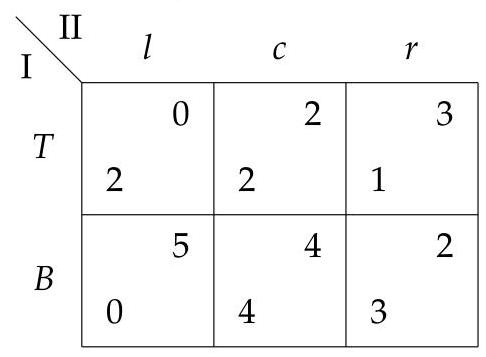
\includegraphics[width=0.5\textwidth]{images/ch08-fig05.jpg}
\end{center}
\hspace*{3em} 

(a) 找出这个博弈在混合(包括纯)策略下的一个均衡。

(b) 找出玩家 I 的一个极大极小策略(可能是混合策略)，以及玩家 I 由此获得的极大极小收益。[提示:将该博弈视为一个给玩家 I 带来收益的零和博弈。]

(c) 找出玩家 II 的一个极大极小策略(可能是混合策略)，以及玩家 II 由此获得的极大极小收益。[提示:将该博弈视为一个给玩家 II 带来收益的零和博弈；注意最大值点和最小值点的角色相反。]

(d) 将 (b) 和 (c) 中玩家 I 和玩家 II 的极大极小收益与 (a) 中任何均衡下他们的收益进行比较。
\end{exercise}